\section{Particles in the heliosphere}

Our heliosphere is an enormous region in space embedded in the \ac{ISM}, which encompasses all solar system planets and extends far beyond even the Kuiper belt. 
It is filled with a thin plasma consisting of various populations of particles, many of which originate from the Sun itself (\autoref{fig:heliospheric_energy_spectrum}). 
The most abundant population is the solar wind, a steady flow of plasma that exits the Sun radially. 
In the near-Earth space, the slow solar wind reaches typical speeds between \SIrange[range-phrase={\,and\,}]{300}{500}{\kilo\meter\per\second}.
Due to its high plasma $\beta$, it carries the solar magnetic field with it and forms the \ac{IMF}.
As the Sun rotates, the \ac{IMF} carried by the solar wind is shaped like an Archimedian spiral, which is named Parker spiral after Eugene N. \citet{Parker-1958}.

\begin{figure}
    \centering
    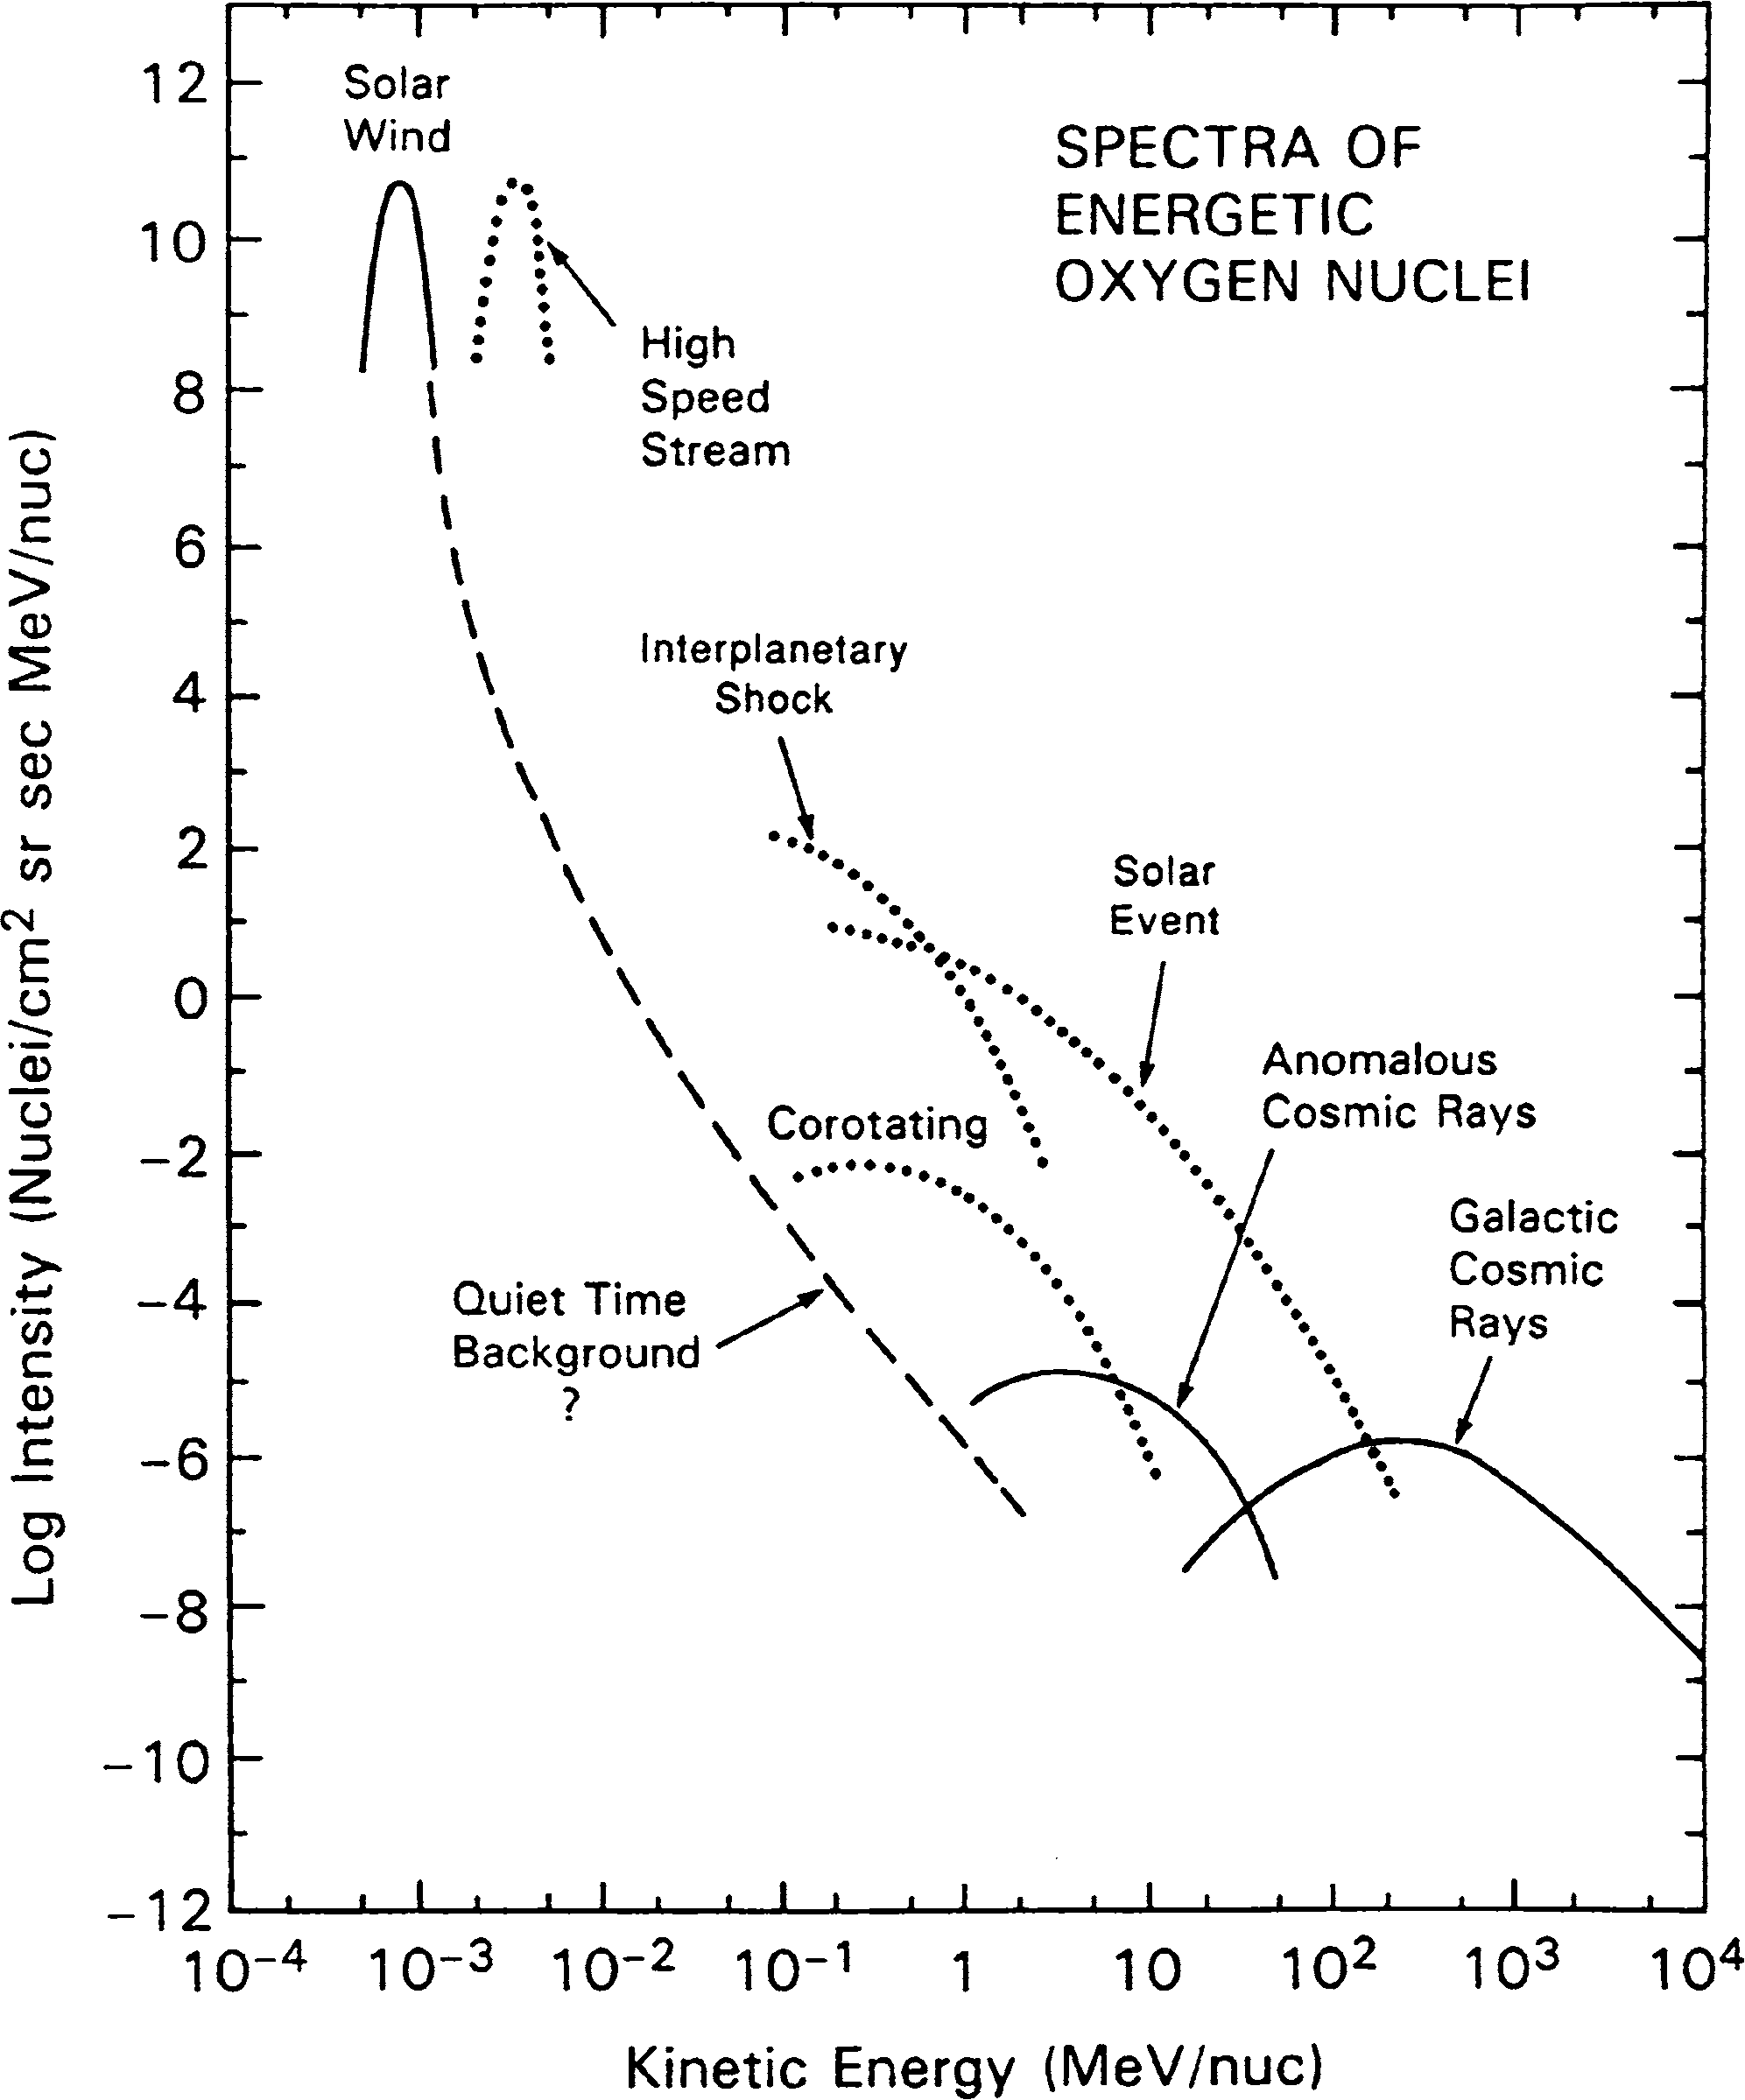
\includegraphics[width=0.6\linewidth]{images/heliospheric_energy_spectrum}
    \caption[Spectra of oxygen ions in the near-Earth interplanetary space]{Typical spectra of oxygen ions in the near-Earth interplanetary space, showing the contributions from different populations. Other particle species show similarly shaped spectra when plotted as a function of energy/nucleon. (adapted from \url{http://helios.gsfc.nasa.gov/ace/gallery.html}).}
    \label{fig:heliospheric_energy_spectrum}
\end{figure}

However, our Sun is an active star, and thus, the flow of particles is not simply constant.
Coronal holes forming on the solar surface emit faster solar wind streams with speeds $\gtrsim \SI{600}{\kilo\meter\per\second}$, which interact with the neighboring streams of slower wind by forming a \ac{SIR}. If a coronal hole stays stable for multiple solar rotations, these interaction regions can be observed recurrently, in which case they are called \acp{CIR}.
Furthermore, active regions can occasionally produce solar flares, sudden and intense emissions of light often associated with the release of high-energy ($\sim \si{\mega\electronvolt}$) \acp{SEP}.
These are believed to be powered by reconnection of magnetic field lines at the Sun, which leads to the release of energy and acceleration of particles.
They often also coincide with the eruption of plasma from the solar corona in the form of a \ac{CME} at speeds up to a few thousands of \si{\kilo\meter\per\second}.

At the high end of the energy spectrum (\autoref{fig:heliospheric_energy_spectrum}) up to \si{\giga\electronvolt} energies, we find \acp{GCR}, particles originating from outside the heliosphere and entering it with a relatively constant and isotropic flux. 
The flux of these high-energy particles within the heliosphere is modulated by various effects: In the long term, the variation of the \ac{IMF} intensity during the 22-year solar cycle causes the average GCR flux to be higher during solar minimum than at solar maximum. In addition, there can be short-term modulations of \ac{GCR} due to magnetic structures in the solar wind, such as \acp{CME} and \acp{SIR}/\acp{CIR}. In the case of observations that are not made in deep space, but on the surface of Earth or other planets, the atmosphere and magnetosphere of this planet also modulates the observed \ac{GCR} spectrum, e.g. by shielding away lower energy particles. 

% TODO: add citations.

\section{Space Weather events}



\section{Forbush decreases}

\section{Motivation}

\ac{MSL}/\ac{RAD}